\documentclass{beamer}
%\documentclass[handout]{beamer}
%\documentclass[handout, notes=show]{beamer}

\usepackage[french]{babel}
\usepackage[utf8]{inputenc}
\usepackage{times}
\usepackage[T1]{fontenc}

\usepackage{graphicx}
\graphicspath{{../report/img/}{./img/}}
\usepackage{hyperref}
\hypersetup{colorlinks=true,linkcolor=red}
\usepackage{pgfpages}
\usepackage{csvsimple}

%\PassOptionsToPackage{subsection=false}{beamerouterthememiniframes}
\mode<presentation>
{
    \hypersetup{pdfpagemode=FullScreen} %FullScreen, None
    \hypersetup{pdfstartpage=12}

    %\usetheme{default}
    %\usetheme{Bergen}
    %\usetheme{Boadilla}
    %\usetheme{CambridgeUS}
    %\usetheme{Antibes}
    %\usetheme{Berkeley}
    \usetheme{Warsaw}
    %\usetheme{Singapore}
    %\usetheme[compress]{Berlin}
    %\usetheme{Copenhagen}

    \usecolortheme[named=darkgray]{structure}

    \setbeamercovered{transparent=10}
    \setbeamertemplate{footline}[frame number]
}

\mode<handout>{
    \hypersetup{pdfpagemode=None}
    \hypersetup{pdfpagelayout=SinglePage}
    \hypersetup{pdfstartview=Fit}

    \pgfpagesuselayout{2 on 1}[a4paper,border shrink=5mm]

    \setbeamercolor{background canvas}{bg=black!5}
    \setbeamertemplate{footline}[frame number]
}

\title[]{Algorithmes avancés}
\subtitle{Clustering et classification supervisée}
\author{Claudio Sousa, David Gonzalez}
\institute{HEPIA}
\date{11/06/2018}

\pgfdeclareimage[width=1cm]{logo}{logo}
\logo{\pgfuseimage{logo}}

\setcounter{tocdepth}{3}

\begin{document}

\begin{frame}[plain]
    \titlepage
\end{frame}

\section{Clustering}

\begin{frame}[plain]
    \begin{figure}[H]
        \begin{center}
            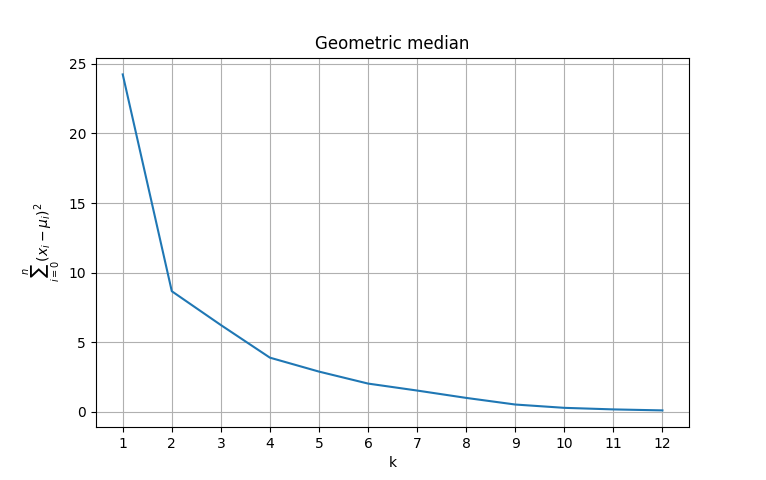
\includegraphics[width=1\textwidth]{ex1_geometric_median}
        \end{center}
        \caption{Distance en fonction de \textit{K}}
        \label{Distance en fonction de K}
    \end{figure}
\end{frame}

\begin{frame}[plain]
    \begin{figure}[H]
        \begin{center}
            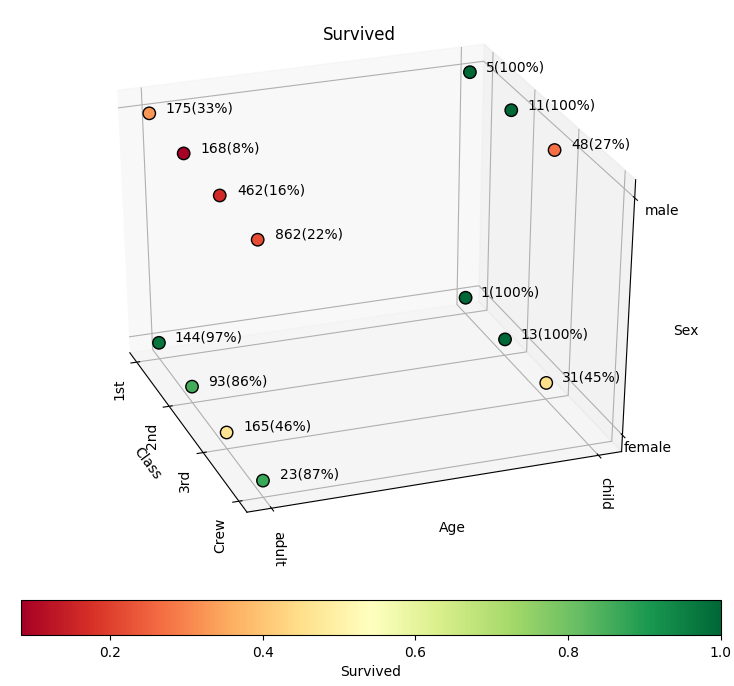
\includegraphics[width=0.75\textwidth]{ex1_survived}
        \end{center}
        \caption{Survie selon paramètres}
        \label{Survie selon paramètres}
    \end{figure}
\end{frame}

\begin{frame}[plain]
    \begin{figure}[H]
        \begin{center}
            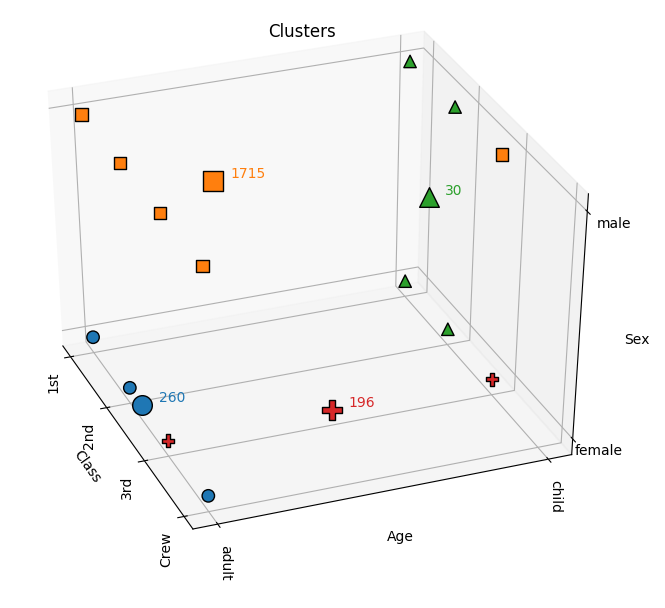
\includegraphics[width=0.75\textwidth]{ex1_clusters}
        \end{center}
        \caption{Clustering $(K=4)$}
        \label{Clustering}
    \end{figure}
\end{frame}

\begin{frame}[plain]
    \begin{figure}[H]
        \begin{center}
            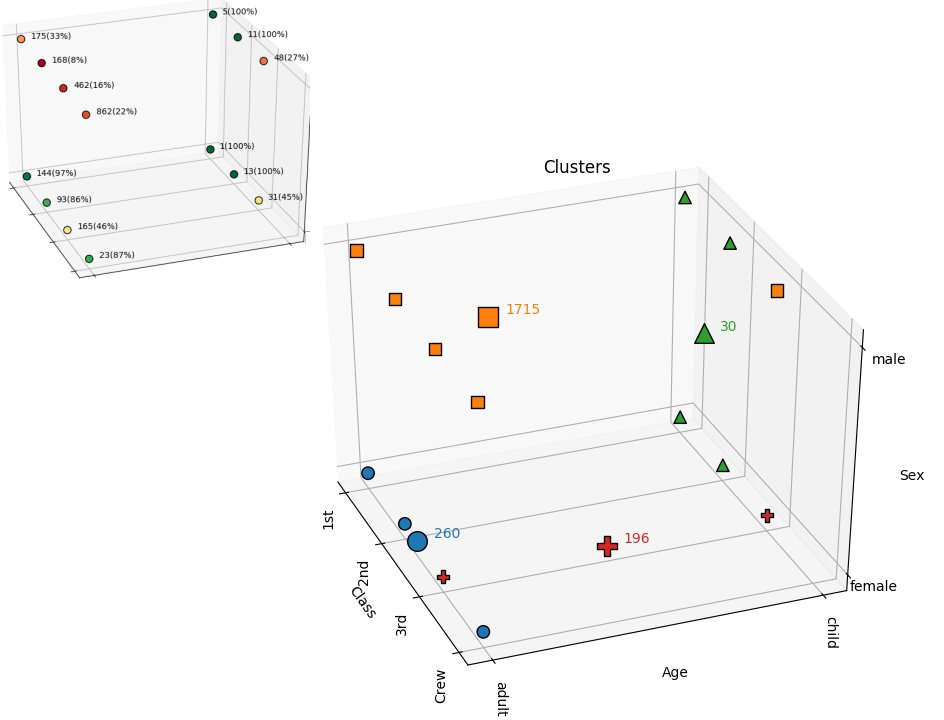
\includegraphics[width=1\textwidth]{survived_clusters}
        \end{center}
        \caption{Clustering $(K=4)$}
        \label{Clustering}
    \end{figure}
\end{frame}



\section{Classification supervisée imposée}

\subsection{Données du cancer du sein}

\begin{frame}[plain]
    \begin{figure}[H]
        \begin{center}
            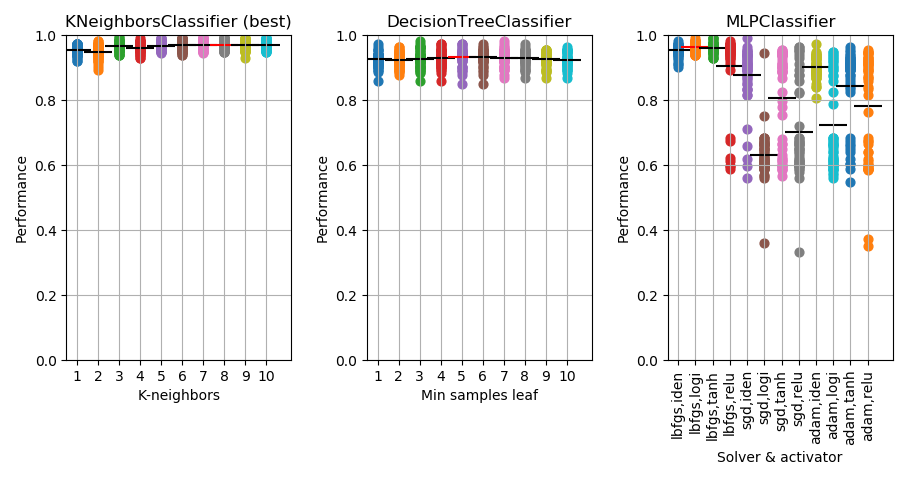
\includegraphics[width=1\textwidth]{ex2_breastcancer}
        \end{center}
        \caption{Résultat de la validation croisée sur les données du cancer du sein}
        \label{Résultat de la validation croisée sur les données du cancer du sein}
    \end{figure}
\end{frame}

\begin{frame}[plain]
    \begin{table}[H]
        \begin{center}
            \csvreader[
                separator=comma,
                head,
                tabular=|l|l|l|l|l|l|,
                table head=\hline \textbf{M1} & \textbf{M2} & \textbf{M3} & \textbf{M4} & \textbf{M5} & \textbf{M6}\\\hline\hline,
                late after line=\\\hline
            ]
            {../report/data/breastcancer.csv}{}
            {\csvcoli & \csvcolii & \csvcoliii & \csvcoliv & \csvcolv & \csvcolvi}
            \csvreader[
                separator=comma,
                head,
                tabular=|l|l|l|l|l|l|,
                table head=\hline \textbf{M7} & \textbf{M8} & \textbf{M9} & \textbf{M10} & \textbf{M11} & \textbf{M12}\\\hline\hline,
                late after line=\\\hline
            ]
            {../report/data/breastcancer.csv}{}
            {\csvcolvii & \csvcolviii & \csvcolix & \csvcolx & \csvcolxi & \csvcolxii}
        \end{center}
        \caption{Résultat de la validation croisée sur les données du cancer du sein}
        \label{Résultat de la validation croisée sur les données du cancer du sein}
    \end{table}
\end{frame}

\subsection{Données des vins}

\begin{frame}[plain]
    \begin{figure}[H]
        \begin{center}
            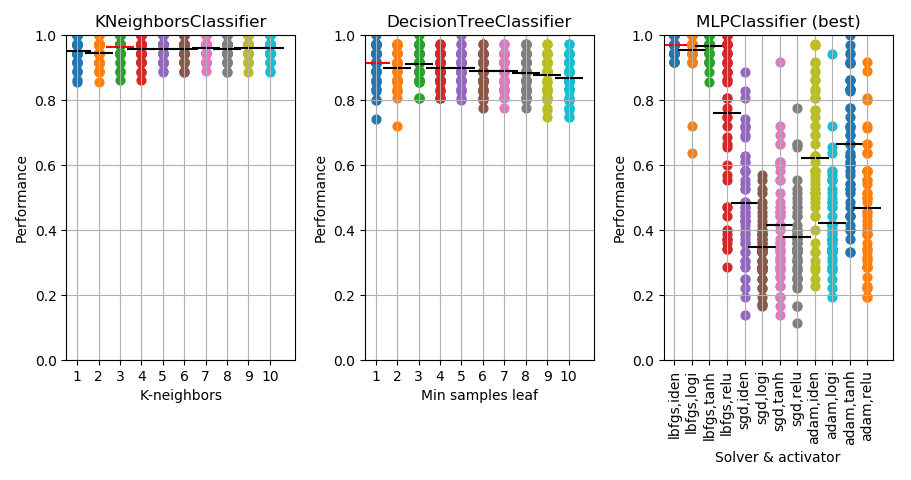
\includegraphics[width=1\textwidth]{ex2_wine}
        \end{center}
        \caption{Résultat de la validation croisée sur les données des vins}
        \label{Résultat de la validation croisée sur les données des vins}
    \end{figure}
\end{frame}

\begin{frame}[plain]
    \begin{table}[H]
        \begin{center}
            \csvreader[
                separator=comma,
                head,
                tabular=|l|l|l|l|l|l|,
                table head=\hline \textbf{M1} & \textbf{M2} & \textbf{M3} & \textbf{M4} & \textbf{M5} & \textbf{M6}\\\hline\hline,
                late after line=\\\hline
            ]
            {../report/data/wine.csv}{}
            {\csvcoli & \csvcolii & \csvcoliii & \csvcoliv & \csvcolv & \csvcolvi}
            \csvreader[
                separator=comma,
                head,
                tabular=|l|l|l|l|l|l|,
                table head=\hline \textbf{M7} & \textbf{M8} & \textbf{M9} & \textbf{M10} & \textbf{M11} & \textbf{M12}\\\hline\hline,
                late after line=\\\hline
            ]
            {../report/data/wine.csv}{}
            {\csvcolvii & \csvcolviii & \csvcolix & \csvcolx & \csvcolxi & \csvcolxii}
        \end{center}
        \caption{Résultat de la validation croisée sur les données des vins}
        \label{Résultat de la validation croisée sur les données des vins}
    \end{table}
\end{frame}

\section{Classification supervisée libre}

\begin{frame}[plain]
    \begin{figure}[H]
        \begin{center}
            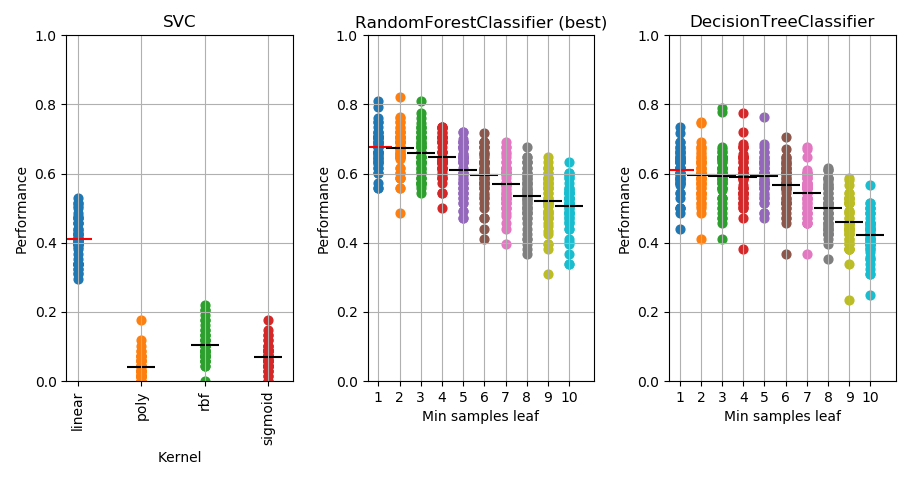
\includegraphics[width=1\textwidth]{ex3}
        \end{center}
        \caption{Résultat de la validation croisée sur les données des feuilles de plantes}
        \label{Résultat de la validation croisée sur les données des feuilles de plantes}
    \end{figure}
\end{frame}

\begin{frame}[plain]
    \begin{table}[H]
        \begin{center}
            \csvreader[
                separator=comma,
                head,
                tabular=|l|l|l|l|l|l|,
                table head=\hline \textbf{M1} & \textbf{M2} & \textbf{M3} & \textbf{M4} & \textbf{M5} & \textbf{M6}\\\hline\hline,
                late after line=\\\hline
            ]
            {../report/data/leaf.csv}{}
            {\csvcoli & \csvcolii & \csvcoliii & \csvcoliv & \csvcolv & \csvcolvi}
            \csvreader[
                separator=comma,
                head,
                tabular=|l|l|l|l|,
                table head=\hline \textbf{M7} & \textbf{M8} & \textbf{M9} & \textbf{M10}\\\hline\hline,
                late after line=\\\hline
            ]
            {../report/data/leaf.csv}{}
            {\csvcolvii & \csvcolviii & \csvcolix & \csvcolx}
        \end{center}
        \caption{Résultat de la validation croisée sur les données des feuilles de plantes}
        \label{Résultat de la validation croisée sur les données des feuilles de plantes}
    \end{table}
\end{frame}

\end{document}
